\documentclass[../defence.tex]{subfiles}
\begin{document}

  \begin{frame}{Landauniveaus II}
    \begin{columns}[onlytextwidth, T]
      \column{\dimexpr\linewidth / 2}
        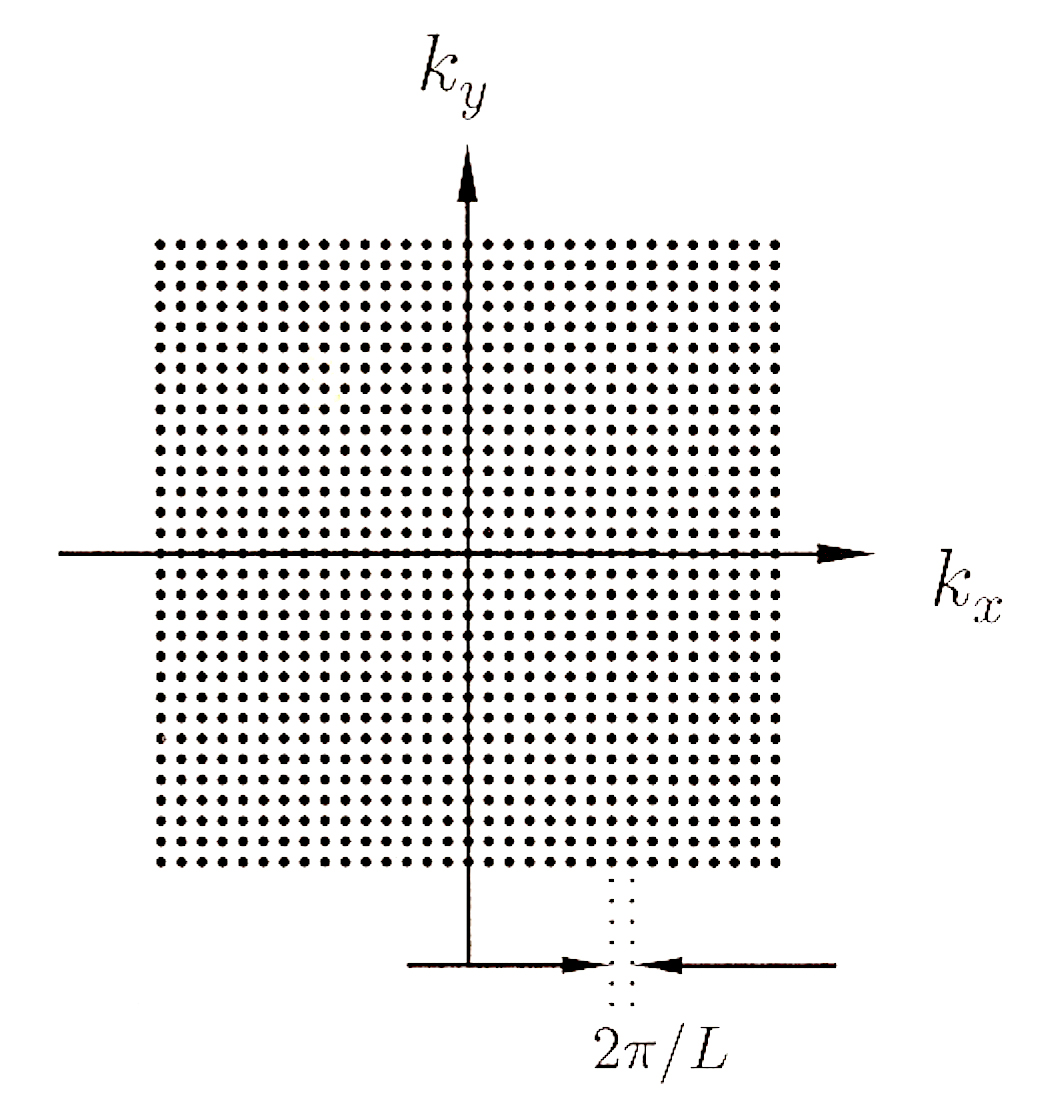
\includegraphics[width=\linewidth]{images/kraum.png}
        \cite{gross}
      \column{\dimexpr\linewidth / 2}
        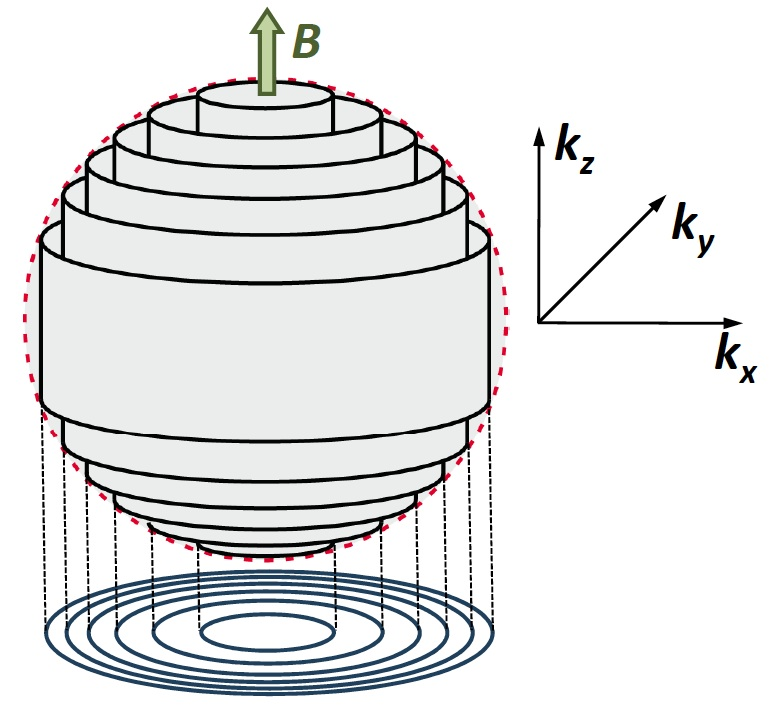
\includegraphics[width=\linewidth]{images/landau_cylinder.png}
        \cite{gross}
    \end{columns}
  \end{frame}
  \note{
  \begin{itemize}
    \item Zustände im $k$-Raum $\rightarrow$ im dreidimensionalen durch Fermi-Kugel beschränkt
    \item Landau-Zylinder im dreidimensionalen $k$-Raum $\rightarrow$ Kreisbahnen mit variablem $k_z$ parallel zum Magnetfeld
  \end{itemize}
  }

\end{document}
